\documentclass[a4paper, twoside]{report}

\usepackage[english]{babel}
\usepackage[utf8]{inputenc}
\usepackage[T1]{fontenc}
\usepackage{listings}
\usepackage{hyperref}
\hypersetup{colorlinks=false}
\usepackage{lscape}
\usepackage{subfigure}
\usepackage{amsmath}
\usepackage{amssymb}
\usepackage{mathrsfs}
\usepackage{graphicx}
\usepackage[colorinlistoftodos]{todonotes}
\usepackage[backend=biber]{biblatex}

\addbibresource{bibs/references.bib}
%% Sets page size and margins
\usepackage[a4paper,top=3cm,bottom=2cm,left=3cm,right=3cm,marginparwidth=1.75cm]{geometry}

\usepackage{ntheorem}

\theoremstyle{break}
\newtheorem{theorem}{Theorem}[section]
\newtheorem{corollary}{Corollary}[theorem]
\newtheorem{lemma}[theorem]{Lemma}
\newtheorem*{problem}{Problem}[section]
\newtheorem*{architecture}{Architecture}[section]


\DeclareMathOperator{\balance}{balance}
\DeclareMathOperator{\argmin}{argmin}
\DeclareMathOperator{\aggregate}{AGGREGATE}
\DeclareMathOperator{\combine}{COMBINE}
\DeclareMathOperator{\readout}{READOUT}
\DeclareMathOperator{\MAX}{MAX}
\DeclareMathOperator{\MEAN}{MEAN}
\DeclareMathOperator{\relu}{ReLU}
\DeclareMathOperator{\concat}{CONCAT}
\DeclareMathOperator{\mlp}{MLP}
\DeclareMathOperator{\hash}{HASH}
\DeclareMathOperator{\gin}{GIN}


\title{Contemplation on \\
{\it Fair Clustering Through Fairlets}}

\author{Junghyun Lee}
% Update supervisor and other title stuff in title/title.tex

\begin{document}
\begin{titlepage}

\newcommand{\HRule}{\rule{\linewidth}{0.5mm}} % Defines a new command for the horizontal lines, change thickness here

%----------------------------------------------------------------------------------------
%	LOGO SECTION
%----------------------------------------------------------------------------------------

\includegraphics[width=8cm]{title/logo.png}\\[1cm] % Include a department/university logo - this will require the graphicx package
 
%----------------------------------------------------------------------------------------

\center % Center everything on the page

%----------------------------------------------------------------------------------------
%	HEADING SECTIONS
%----------------------------------------------------------------------------------------
\quad\\[1.5cm]
%\textsc{\LARGE MSc Thesis}\\[1.5cm] % Name of your university/college
\textsc{\Large Korea Advanced Institute of Technology}\\[0.5cm] % Major heading such as course name
\textsc{\large Department of Mathematical Sciences}\\[0.5cm] % Minor heading such as course title

%----------------------------------------------------------------------------------------
%	TITLE SECTION
%----------------------------------------------------------------------------------------
\makeatletter
\HRule \\[0.4cm]
{ \huge \bfseries \@title}\\[0.4cm] % Title of your document
\HRule \\[1.5cm]
 
%----------------------------------------------------------------------------------------
%	AUTHOR SECTION
%----------------------------------------------------------------------------------------

\begin{minipage}{0.4\textwidth}
\begin{flushleft} \large
\emph{Author:}\\
\@author % Your name
\end{flushleft}
\end{minipage}
~
\begin{minipage}{0.4\textwidth}
\begin{flushright} \large
\emph{Instructor:} \\
Prof. Chang Dong Yoo 
% Uncomment the following lines if there's a co-supervisor
%\\[1.2em] % Supervisor's Name
%\emph{Co-Supervisor:} \\
%Dr. Adam Smith % second marker's name
\end{flushright}
\end{minipage}\\[3cm]
\makeatother


%----------------------------------------------------------------------------------------
%	DATE SECTION
%----------------------------------------------------------------------------------------

{\large Homework \#4}\\[0.5cm]
{\large \emph{EE531: Statistical Learning Theory, Fall 2019}}\\[0.5cm]
{\large \today}\\[2cm] % Date, change the \today to a set date if you want to be precise

\vfill % Fill the rest of the page with whitespace

\end{titlepage}

\begin{abstract}
This writing is an extensive outline of the paper {\it How powerful are graph neural networks?} by Xu {\it et al.}, including summaries of the theorems/lemmas and additional explanation on some of the literatures/points that the paper omitted.

(This is to be accompanied by the pdf file used in the final presentation. Also, the theorem/lemma/corollary numbering is arbitrary, but the statements are exact.)
\end{abstract}

\tableofcontents
\listoffigures

\chapter{Introduction}

\section{Motivation}

Machine learning is becoming ubiquitous in our life; from self-driving car to drug prediction in chemistry, it is becoming part of our life. It is possible that the algorithms, though they aren't inherently biased, may pick up and amplify biases already present in the training data.
Thus a recent line of work has emerged on the {\it fairness} of some of these machine learning algorithms.

Many different notions of fairness have been studied. (Refer to \cite{Mehrabi2019}\cite{Zhong2019} for a survey of fairness)
Here we'll be focused on the notion of {\bf disparate impact}.
Since {\bf Griggs v. Duke Power Co.}\cite{Griggs1971}, disparate impact has earned its place as one of the fundamental rules for fair employment in the U.S. laws. Most notably, the $80\%$-rule\cite{Biddle2006} is the direct result of this.
According to \cite{uniform}, disparate impact is {\it substantially different rate of selection in hiring, promotion, or other employment decision which works to the disadvantage of members of a race, sex, or ethnic group}.

This work answers the question of how to formalize this notion of disparate impact in the context of clustering problem, and how to actually solve it in that framework.


\section{Previous / Related Works}

Currently, there are two "big" tracks in fairness research:
\begin{itemize}
	\item Codifying the meaning of fairness in algorithms
	\item Modifying algorithms to make it achieve fair outcomes under a specific notion of fairness
\end{itemize}

In the case of disparate impact, Feldman {\it et al.}\cite{Feldman2015} did some work in the first track. This work, on the other hand, is closer to the second track, and is one of the first in the unsupervised learning tasks.
Unlike other works, {\it strong guarantees} on the quality of any fair clustering solution.


The general framework of this work follows that of Zemel {\it et al.}\cite{Zemel2013}. Instead of trying to modify an existing algorithm to be fair, our goal here is try to {\bf learn a set of intermediate representations to satisfy two competing goals:}
\begin{itemize}
	\item The intermediate representation should encode the data as well as possible.
	\item The encoded representation is sanitized in the sense that it should be {\bf blind to whether or not the individual is from the protected group}.
\end{itemize}
    
Under this framework, any classification algorithm can be transformed into a fair classifier, by simply {\it applying the classifer to the sanitized representation of the data}.


This work is also closely related to that of Zafar {\it et al.}\cite{Zafar2017}.  Part of their work was focused on designing a convex margin-based classifier that maximizes accuracy subject to fairness constraints, and helps ensure compliance with a non-discrimination policy or law (e.g., a given $p\%$-rule)
This work addresses an open question in that work, which asked for a general framework to solve an unsupervised learning task respecting the $p\%$-rule.
\chapter{Preliminaries}

\section{GNNs}

Consider a graph, $G = (V, E)$, or a data with graph structure. Then each node $v \in V$ is associated with a {\it node feature vector}, denoted as $X_v$.
There are two tasks of interest where GNN is commonly used:

\begin{problem}[Node Classification Problem]
Each $v \in V$ has an associated label $y_v$.

\noindent{\bf Goal:} Learn a representation vector $h_v$ of $v$ such that $y_v = f(h_v)$ i.e. such that $v$'s label can be predicted.
\end{problem}


\begin{problem}[Graph Classification Problem]
A set of graphs $\{G_1, \dots, G_N\} \subset \mathcal{G}$ is given, along with their labels $\{y_1, \dots, y_N\} \subset \mathcal{Y}$.

\noindent{\bf Goal:} Learn a representation vector $h_G$ of $G$ such that $y_G = f(h_G)$ i.e. such that $G$'s label can be predicted. 
\end{problem}


Modern GNNs follow a {\bf neighborhood aggregation strategy} (message passing strategy) in which it iteratively updates the representation of a node by aggregating representations of its neighbors.

Denote $h_v^{(k)}$ as the feature vector of node $v$ at the $k$-th iteration/layer, and let us initialize it as $h_v^{(0)} = X_v$.
Then in this framework, the $k$-th layer of a GNN can be written as

	$$a_v^{(k)} = \aggregate^{(k)} \left( \left\{ h_u^{(k - 1)} : u \in \mathcal{N}_G(v) \right\} \right)$$
	$$h_v^{(k)} = \combine^{(k)} \left( h_v^{(k - 1)}, a_v^{(k)} \right)$$

Different choices of $\aggregate^{(k)}$ and $\combine^{(k)}$ have led to different GNN variants/architectures.

\begin{architecture}[GraphSAGE\cite{Hamilton2017}]
	$$a_v^{(k)} = \MAX \left( \left\{ \relu \left( W h_u^{(k - 1)} \right) : u \in \mathcal{N}_G(v) \right\} \right)$$
	$$h_v^{(k)} = W \left[ h_v^{(k - 1)}, a_v^{(k)} \right]$$
\end{architecture}

\begin{architecture}[Graph Convolutional Networks(GCN)\cite{Kipf2017}]
	$$h_v^{(k)} = \relu \left( W \MEAN \left\{ h_u^{(k - 1)} : u \in \mathcal{N}_G(v) \cup \{v\} \right\} \right)$$
\end{architecture}


Observe that for node classification tasks, the final node representation $h_v^{(K)}$ is directly used for prediction.
However for graph classification tasks, this is not the case i.e. some additional work has to be done to "process" the final node representation to obtain the entire graph's representation.
This is done by aggregating the final node representations by $\readout$ function:
	$$h_G = \readout \left( \left\{ h_v^{(K)} : v \in V \right\} \right)$$ 
	
($\readout$ can be a simple permutation invariant function, or something more sophisticated\cite{Ying2018}\cite{Zhang2018})

%---------------------------------------------------------

\section{WL test}

Now consider the following problem:

\begin{problem}[\textsc{Graph Isomorphism (GI)}]
{\bf Input}:  Two finite graphs $G_1$ and $G_2$

\noindent{\bf Question}: $G_1 \cong G_2$?
\end{problem}

This ubiquitous problem appears everywhere: from mathematical logic, theory of computation, machine learning, to seemingly unrelated fields such as computer vision.
And this seemingly harmless problem has harassed researchers for decades!


It is currently known that \textsc{GI} can be solved in quasipolynomial time {\it i.e.} in $O \left( 2^{O \left( \left( \log n \right)^c \right)} \right) (c > 0)$ time\cite{Babai2016}.
The precise statement is as follows:
	
\begin{theorem}[Babai, 2015]
The Graph Isomorphism problem ... can be solved in quasipolynomial time.
\end{theorem}

But this is not practical.
In practice, other less efficient algorithms are used, such as algorithms by McKay (1981), Schmidt \& Druffel (1976), Ullman (1976)...etc.


Here, we shall talk about one specific combinatorial algorithm for \textsc{GI}: the Weisfeiler-Lehman test of graph isomorphism\cite{Weisfeiler1968}, or simply WL test.

WL test is proved to be successful (and computationally efficient) in isomorphism testing for a broad class of graphs\cite{Babai1979} There are some (corner) cases (ex. regular graphs) when the WL test fails\cite{Cai1992}.

The reason the people working on GNNs got so interested in the WL test is that its 1-dimensional form (a.k.a. "na\"ive vertex refinement") is {\it based on neighbor aggregations}, analogous to the GNNs!
(And that is why we'll be focused only on the 1-dim case)

Let $(G, l)$ be a labeled graph i.e. a graph $G$ with an endowed node coloring $l : V(G) \rightarrow \Sigma$.
($\Sigma$: arbitrary codomain)
Here is the full algorithm for the 1-dim WL test\cite{Shervashidze2009}:

\begin{figure}[hbt]
\centering
	\includegraphics[height=7cm]{preliminaries/fig/wl-alg.png}
	\caption{One iteration of 1-dim WL test}
\end{figure}
	(This why this 1-dim version is commonly called the {\it color refinement algorithm})

To relate this to GNN, we need one more concept; graph kernel.

Graph kernel is a kernel function that defines {\it inner product on graphs} \cite{Vishwanathan2010}.
Intuitively, it is a function that measures the similarity of a pair of two given graphs.
There are many different variants of graph kernels, but we'll be focused on the Weisfeiler-Lehman subtree kernel\cite{Shervashidze2009}.
(Refer to \cite{Vishwanathan2010} for a extensive study of graph kernels and \cite{Shervashidze2011} for a more thorough explanation of the WL subtree kernel)

The WL subtree kernel counts common {\it original and compressed labels} i.e. common multiset strings in two graphs, resulting from 1-dim WL test.
Below shows the algorithm for calculating the WL subtree kernel:

\begin{figure}[hbt]
\centering
	\includegraphics[height=6cm]{preliminaries/fig/wl-kernel-alg.png}
	\caption{One iteration of WL subtree kernel}
\end{figure}

And below figure is a visualization of one run of the WL subtree kernel:

\begin{figure}[hbt!]
\centering
	\includegraphics[height=13cm]{preliminaries/fig/fig1.png}
	\caption{Illustration of the computation of the WL subtree kernel (with respect to one iteration) for two graphs}
\end{figure}

\newpage
\section{(Overview of) Theoretical Framework}

In other words, the WL subtree uses the counts of node labels at different iterations of the WL test as the feature vector of a graph.
Intuitively, a node’s label at the $k$-th iteration of the 1-dim WL test represents a {\bf subtree structure of height k rooted at the node}.

Thus, the graph features considered by the WL subtree kernel are essentially counts of different rooted subtrees in the graph!

\begin{figure}[hbt!]
\centering
	\includegraphics[height=4cm]{preliminaries/fig/fig2.png}
	\caption{An overview of the theoretical framework}
\end{figure}

What this tells us is that if a GNN's aggregation function captures the {\it full multiset} of node neighbors, the GNN can capture the rooted subtrees in a recursive manner and be as powerful as the WL test (as shown in above figure).

To analyze the representational power of a GNN, we ask ourselves the question: {\it when does a GNN map two nodes to the same location in the embedding space)? }
{\bf Intuitively, a maximally powerful GNN maps two nodes to the same location only if they have identical subtree structures with identical features on the corresponding nodes.}
Since subtree structures are defined recursively via node neighborhoods (above figure), we can reduce our analysis to the question whether a GNN maps two neighborhoods (i.e., two multisets) to the same embedding or representation.
A maximally powerful GNN would never map two different neighborhoods, i.e., multisets of feature vectors, to the same representation.
This means its aggregation scheme must be injective. Thus, we abstract a GNN’s aggregation scheme as a class of functions over multisets that their neural networks can represent, and analyze whether they are able to represent injective multiset functions.

(Above paragraph is taken directly from the paper because it is the key point in this whole work!)

\chapter{Results}
%For my evaluation, I've used {\bf Tensorboard} for plotting the learning(loss) curve and performance(accuracy) curve for both training and validating processes. Also, I've used external open source library({\bf pretty-print-confusion-matrix}\footnote{\url{https://github.com/wcipriano/pretty-print-confusion-matrix}}) for plotting the confusion matrix for the test set.
Here,
\begin{itemize}
\item Original model: One with uniform initialization with dropouts(rate=0.5).

\item Ver. 1: Original model with Xavier (Uniform) Initialization

\item Ver. 2: Original model without dropouts

\item Ver. 3: Original model with Xavier Initialization and without dropouts
\end{itemize}

In all the plots, x-axis corresponds to the epoch.
As for the graphs,

\begin{itemize}
\item Accuracy graph
	\begin{itemize}
	\item Dark red: train accuracy
	\item Bright red: validation accuracy
	\end{itemize}

\item Loss graph
	\begin{itemize}
	\item Dark blue: train loss
	\item Bright blue: validation loss
	\end{itemize}
\end{itemize}

\newpage
\section{Original model}

\begin{figure}[htbp]
\centering
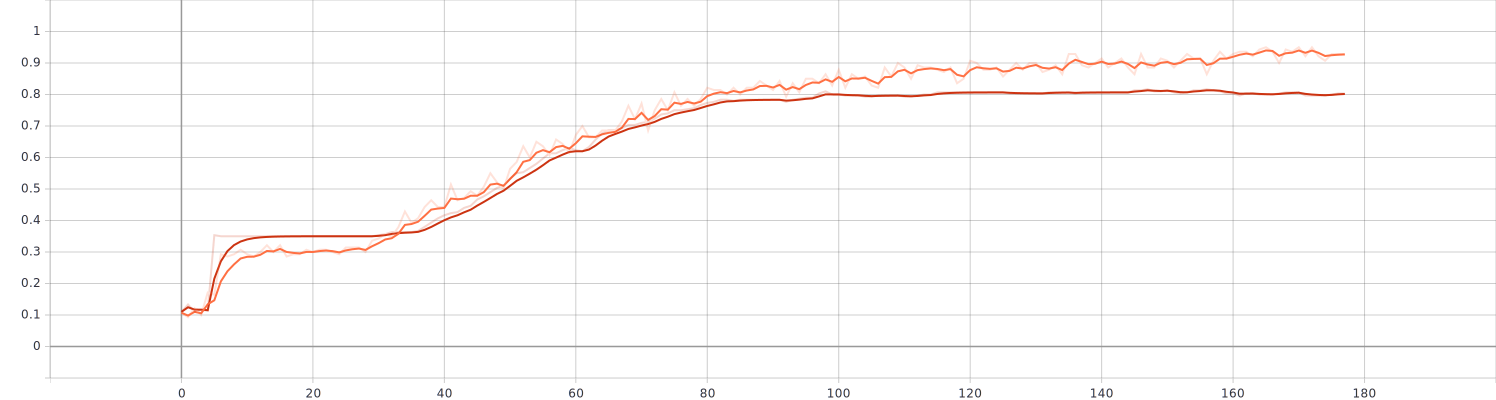
\includegraphics[width=0.7\linewidth]{results/fig/Accuracy0.png}
\caption{Accuracy graph}
\label{fig:accuracy0}
\end{figure}

\begin{figure}[htbp]
\centering
\includegraphics[width=0.7\linewidth]{results/fig/Loss0.png}
\caption{Loss graph}
\label{fig:evaluation0}
\end{figure}

\begin{figure}[htbp]
\centering
\includegraphics[width=0.6\linewidth]{results/fig/confusion0.png}
\caption{Confusion matrix}
\label{fig:confusion0}
\end{figure}

\newpage
\section{Modified Model (Ver. 1)}

\begin{figure}[htbp]
\centering
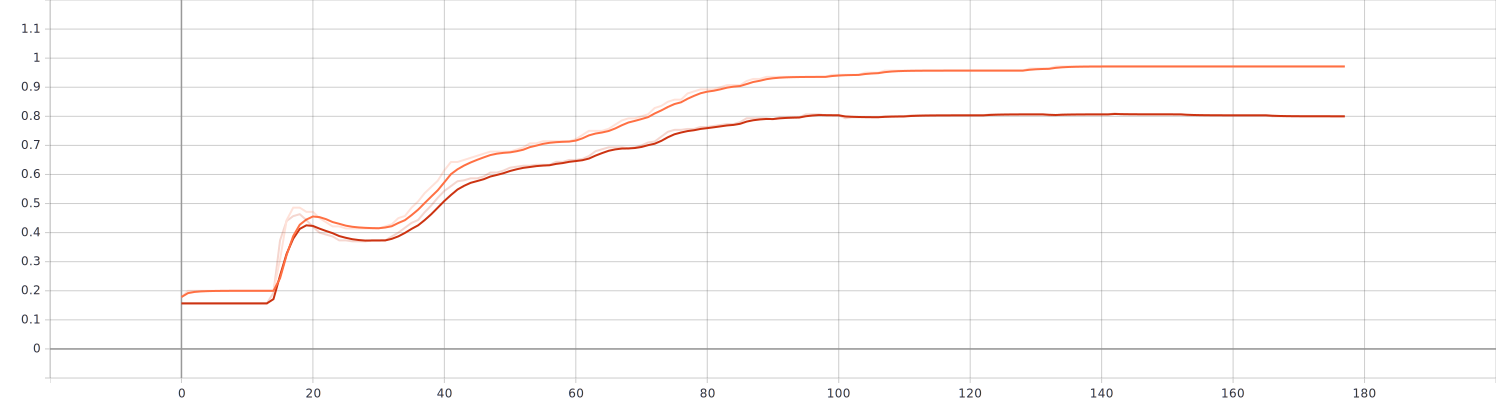
\includegraphics[width=0.7\linewidth]{results/fig/Accuracy1.png}
\caption{Accuracy graph}
\label{fig:accuracy1}
\end{figure}

\begin{figure}[htbp]
\centering
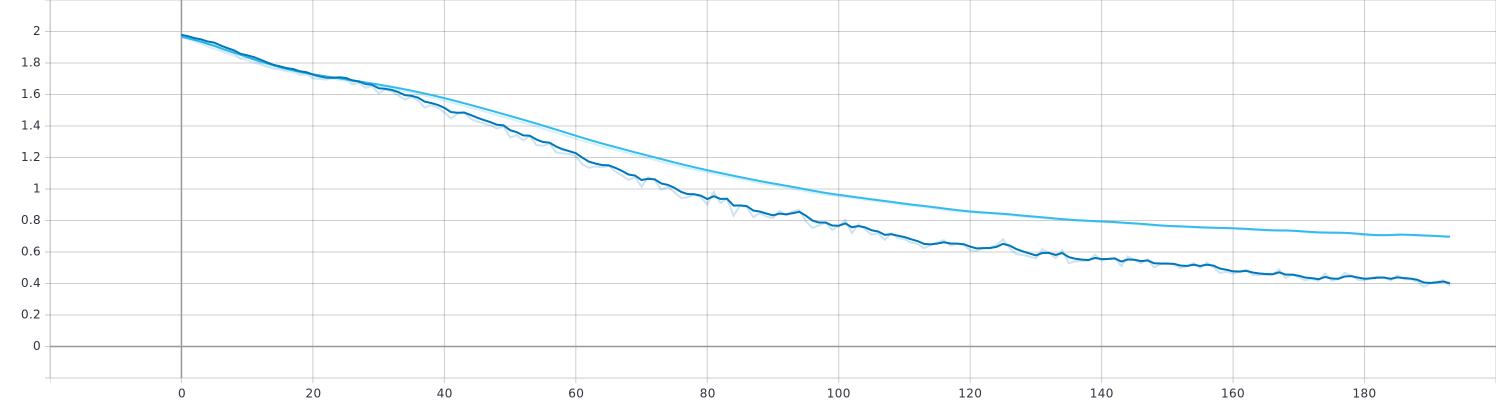
\includegraphics[width=0.7\linewidth]{results/fig/Loss1.png}
\caption{Loss graph}
\label{fig:evaluation1}
\end{figure}

\begin{figure}[htbp]
\centering
\includegraphics[width=0.6\linewidth]{results/fig/confusion1.png}
\caption{Confusion matrix}
\label{fig:confusion1}
\end{figure}

\newpage
\section{Modified Model (Ver. 2)}

\begin{figure}[htbp]
\centering
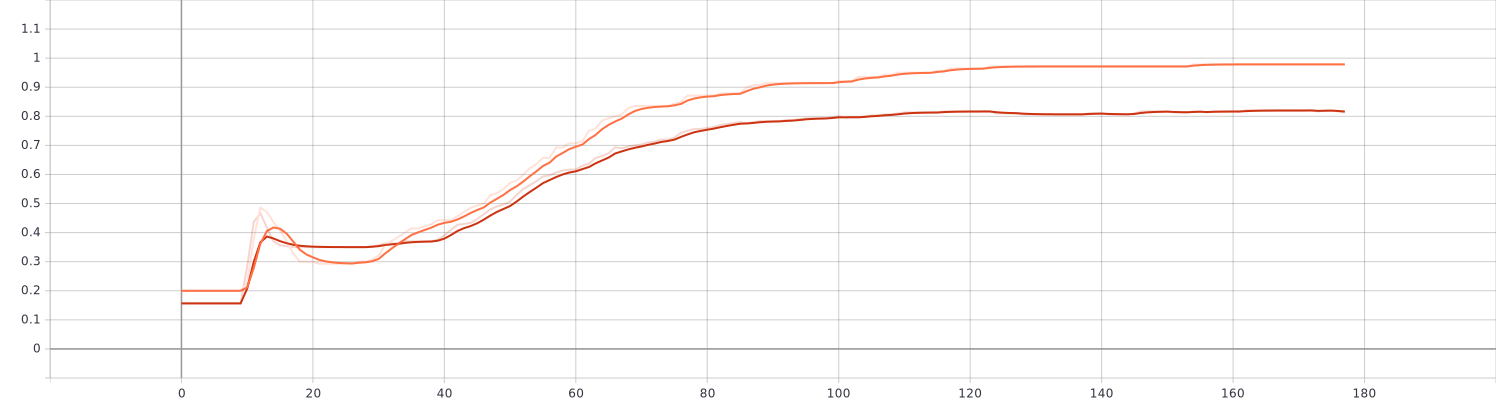
\includegraphics[width=0.7\linewidth]{results/fig/Accuracy2.png}
\caption{Accuracy graph}
\label{fig:accuracy2}
\end{figure}

\begin{figure}[htbp]
\centering
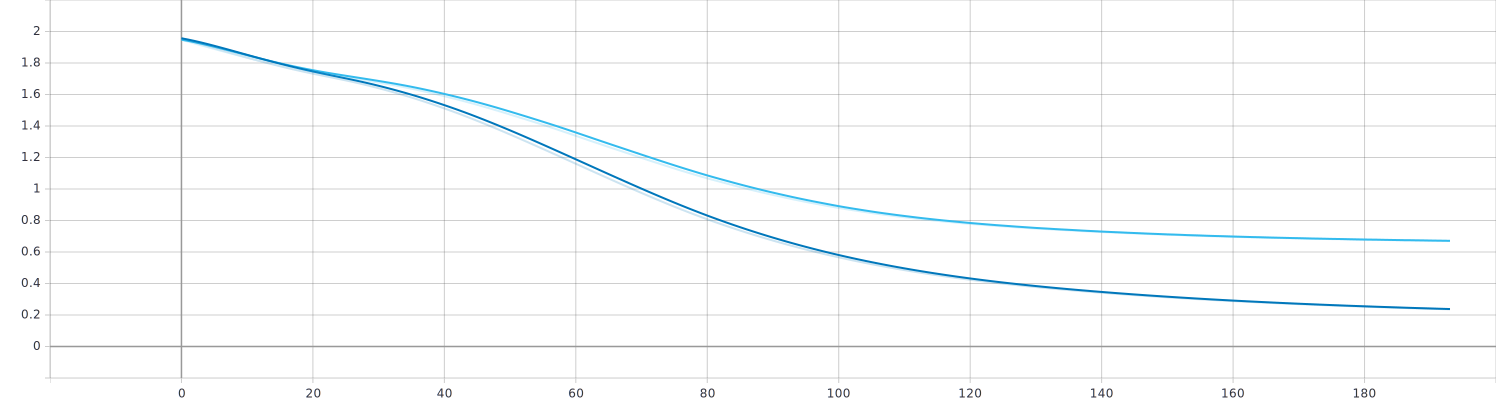
\includegraphics[width=0.7\linewidth]{results/fig/Loss2.png}
\caption{Loss graph}
\label{fig:evaluation2}
\end{figure}

\begin{figure}[htbp]
\centering
\includegraphics[width=0.6\linewidth]{results/fig/confusion2.png}
\caption{Confusion matrix}
\label{fig:confusion2}
\end{figure}

\newpage
\section{Modified Model (Ver. 3)}

\begin{figure}[htbp]
\centering
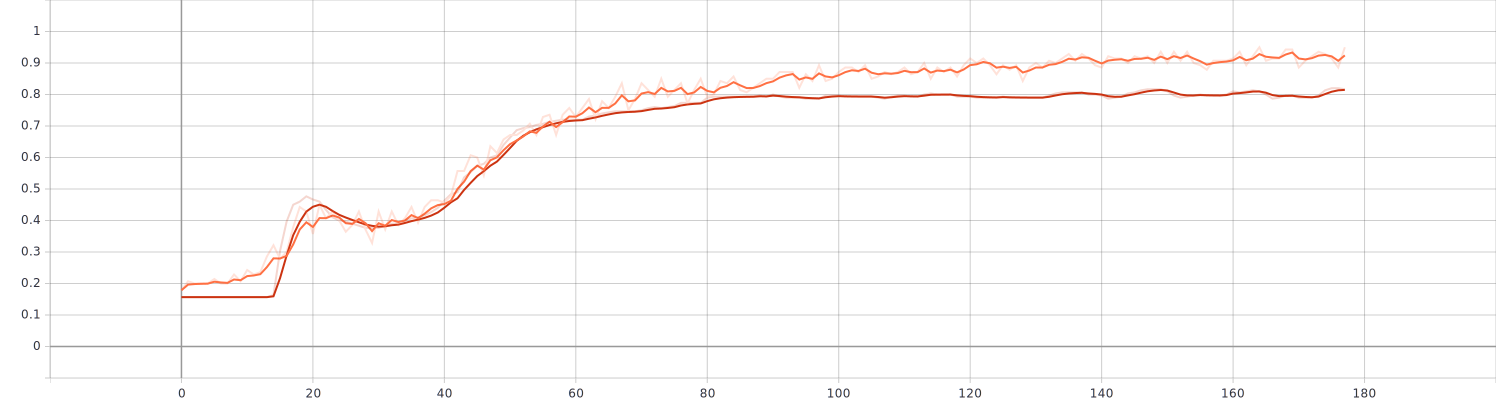
\includegraphics[width=0.7\linewidth]{results/fig/Accuracy3.png}
\caption{Accuracy graph}
\label{fig:accuracy3}
\end{figure}

\begin{figure}[htbp]
\centering
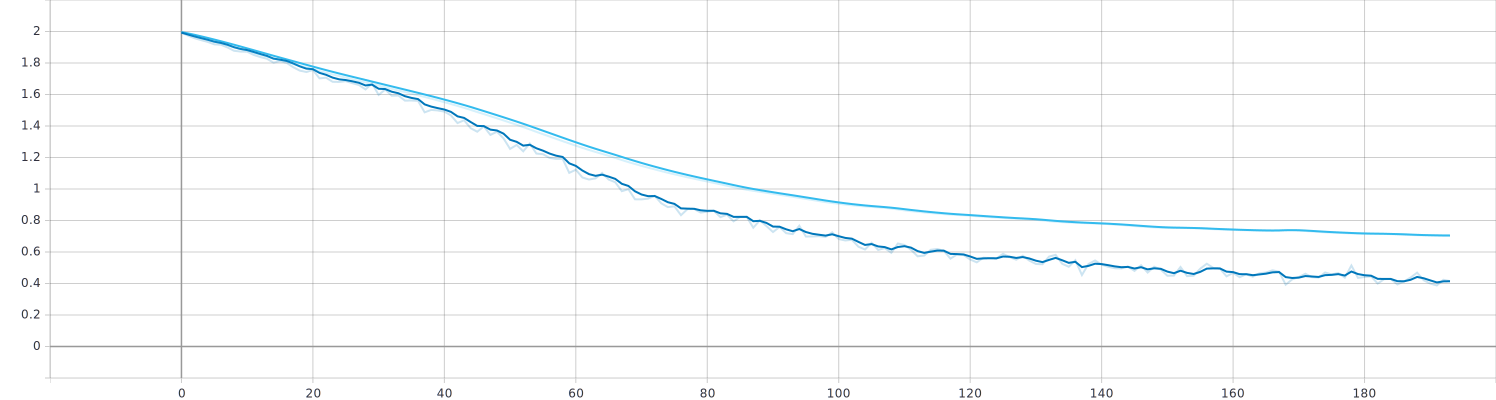
\includegraphics[width=0.7\linewidth]{results/fig/Loss3.png}
\caption{Loss graph}
\label{fig:evaluation3}
\end{figure}

\begin{figure}[htbp]
\centering
\includegraphics[width=0.6\linewidth]{results/fig/confusion3.png}
\caption{Confusion matrix}
\label{fig:confusion3}
\end{figure}

\chapter{Experiments}

The goal of the experiments is two-fold:

\begin{itemize}
	\item Show that the traditional algorithms for $k$-center and $k$-median tend to produce unfair clusters

	\item Show that the proposed algorithm outputs clusters that respect the fairness guarantees
\end{itemize}


\section{Experiment Design}

3 datasets from \cite{Lichman2013} were used:
\begin{itemize}
	\item Diabetes (gender)
	\item Bank (married or not married)
	\item Sensus (gender)
\end{itemize}

The atttributes in the parenthesis are the protected attributes for each one. The unprotected attributes were chosen as the numeric attributes such as age, capital-gain...etc. (different for each dataset)

As for the algorithm, the flow-based fairlet decomposition algorithm (as discussed previously) was implemented.
For the vanilla $k$-center clustering algorithm, the {\it greedy furthest point algorithm\cite{Gonzalez1985}} was used.
For the vanilla $k$-median clustering algorithm, {\it single swap algorithm\cite{Arya2004}} was used. The reason for this choice, even though it obtains 5-approximation in the worst case, is that it performs well in practice. (Refer to Kanungo {\it et al.}, 2002) for more information.)

In all cases, the experiment was done with $t' = 2$ i.e. aiming for balance of at least $0.5$ in each cluster.

\newpage
\section{Results / Analysis}

\begin{figure}[hbt!]
\centering
  \includegraphics[height=7cm]{experiments/fig/fig4.png}
  \caption{Empirical performance of the classical and fair clustering median and center algorithms on the three datasets. The cost of each solution is on left axis, and its balance on the right axis.}
\end{figure}

Observe that as expected, the balance of the solutions produced by the classical algorithms is very low. More than half of the cases show the phenomenon of balance being at 0 for high value of $k$.

On the other hand the fair clustering solutions maintain a balanced solution, regardless of the value of $k$. Not surprisingly, the balance comes with a corresponding increase in cost, and the fair solutions are costlier than
their unfair counterparts.
In all of the scenarios the overall cost of the clustering converges
to the cost of the fairlet decomposition, which serves as a lower bound on the cost of the optimal solution.
\chapter{Conclusion}

It seems that the slight modifications that I've tried did nothing to improve the model's accuracy. Indeed, the original model reports accuracy of 78.40\%, which tied with Ver. 2 and is strictly greater than the other two versions.

This accuracy is actually lower than the reported accuracy from Kipf \& Welling, which is actually 81.5\%.
I can't really explain why this is the case... But one guess is that maybe getting rid of the bias term might increase the accuracy? (<-- just a wild guess)

One interesting observation is that Ver. 3, the model with the most complexity out of the 4 tested, performed the worst with accuracy 77.54\%. It shows that adding in feature/model complexity doesn't always increase the accuracy; it might even decrease it!
%\input{appendix/appendix.tex}

%1. Note that being powerful entails “being able to” map nodes with different subtrees to different representations. If a model is not capable of achieving this, then it’s intrinsically less powerful in distinguishing different graphs. In addition, to combat noise, we can simply regularize the mapping function to be locally smooth (e.g., by using Virtual Adversarial Training [1]). Nonetheless, in many graph classification applications including those in our experiments, the node features have specific meanings (e.g. an atom of certain types) and are not noisy.


\printbibliography
%\bibliographystyle{unsrt}
%\bibliography{bibs/references}
\addcontentsline{toc}{chapter}{Bibliography}

\end{document}